\chapter{Half-plane with Robin boundary} \label{chapter-robin}
In this chapter we will examine the Landau Hamiltonian of a particle confined to a half-plane with a Robin (or \textit{mixed}) boundary condition.
\begin{defn}[Landau Hamiltonian in half-plane with Robin boundary]
    \label{defn-hamiltonian-robin}
    \ph{.}\\
    Let $\alpha \in \R$ and $\Omega := \R \times \R_+$, where $\R_+ \equiv [0, +\infty)$. The Hamiltonian is given by\footnote{
    The equalities are to be understood in the weak sense again. $(H_\alpha \psi)(x, y) = ...$ holds for almost every $(x,y)$ in $\Omega$ with respect to the Lebesgue measure. $\psi(0,y) \equiv \lim_{x \to 0} \psi(x,y) = ...$ holds for almost every $y\in\R$, and the limit is the \textit{essential} limit wrt. the Lebesgue measure.
}
\begin{equation}
    \begin{gathered}
        \big( H_\alpha \psi \big)(x,y)
        = \left(
            -\pd{^2}{x^2} +
            \big( {-\i} \pd{}{y} + bx \big)^2
        \right) \, \psi(x,y) \: ,
        \\
        \Domain(H_\alpha)
        = \big\{ \,
            \psi \in W^{2,2}(\Omega) \cap L^2_{x^4}(\Omega)
            \; \big| \;
            \alpha \, \psi(0,y) + \psi'(0,y) = 0
        \, \big\} \: .
    \end{gathered}
\end{equation}
\end{defn}
Using \eqref{eqn-vague-direct-integral-decomp}, we can once again show that the Hamiltonian is unitarily equivalent to a direct integral $H_\alpha \simeq \int^\oplus_\R \Hf_\alpha(p) \d{p}$, where $\Hf(p)$ is the fibre Hamiltonian given by
\begin{equation}
    \begin{gathered}
        \big( \Hf_\alpha(p) \varphi \big)(x)
        = -\varphi''(x) + (p + bx)^2 \, \varphi(x) \: ,
        \\
        \Domain( \Hf_\alpha(p) )
        = \big\{ \,
            \varphi \in W^{2,2}(\R_+) \cap L^2_{x^4}(\R_+)
            \; \big| \;
            \alpha \, \varphi(0) + \varphi'(0) = 0
        \, \big\} \: .
    \end{gathered}
\end{equation}
When $\alpha=0$, the problem reduces to the Neumann boundary condition.

\medskip

The Robin boundary condition is a generalization of the Dirichlet and Neumann boundary conditions. In their article\footnote{To the author's knowledge, the article has not been published in any journal yet.}, \cite{Allwright2016} argued that the Robin b.c. should be viewed as the generic boundary condition for long-wavelength approximations of short-ranged potentials. They give several examples where the characteristic length $L$ of a potential leads to a Robin boundary with $\alpha = 1/L$ in the long-wavelength limit.


\section{Well-posedness}
We will start by showing that the Hamiltonian is bounded from below, starting with the fibre Hamiltonian:
\begin{align*}
    \\[-2\baselineskip]
    \big( \varphi, \Hf_\alpha(p) \, \varphi \big)
    &= - \int_{\R_+} \!\! \overline\varphi \varphi''
    + \overbrace{\int_{\R_+} \! (bx + p)^2 \, |\varphi|^2}^{\geq 0}
    \\
    &\geq -\big[ \overline\varphi \varphi' \big]_0^{\infty}
    + \int_{\R_+} |\varphi'|^2
    \;=\;
    \overline{ \varphi(0) } \, \varphi'(0)
    + \norm{ \varphi' }_{L^2(\R_+)}^2
\end{align*}
We have used integration by parts and the fact that for $\varphi \in W^{2,2}$ both $\varphi$ and $\varphi'$ vanish at infinity. We substitute for $\varphi'(0) = -\alpha \, \varphi(0)$ from the boundary condition:
\begin{align*}
    \big( \varphi, \Hf_\alpha(p) \, \varphi \big)
    \geq \overline{ \varphi(0) } \, \varphi'(0)
    + \norm{ \varphi' }_{L^2(\R_+)}^2
    = - \alpha \, \big| \varphi(0) \big|^2
    + \norm{ \varphi' }_{L^2(\R_+)}^2
    \: .
\end{align*}
For~$\alpha \leq 0$, the whole right-hand side is non-negative. For~$\alpha > 0$, we have:
\begin{align*}
    &\big( \varphi, \Hf_\alpha(p) \, \varphi \big)
    \geq - \alpha \, \big| \varphi(0) \big|^2
    + \norm{ \varphi' }_{L^2(\R_+)}^2
    \geq -\alpha \norm{\varphi}_{L^{\!\infty}(\R_+\!)}^2
    \! + \norm{ \varphi' }_{L^2(\R_+\!)}^2
    \: .
\end{align*}
Now using the lemma \ref{lemma-sobolev-type-inequality} from the Appendix, we know that for every $a>0$ there exists $b>0$ such that $-\alpha \norm{\varphi}_{L^{\!\infty}}^2 \geq -a \, \alpha \norm{\varphi'}_{L^2}^2 - b \, \alpha \norm{\varphi}_{L^2}^2$. Setting $a = \alpha^{-1}$, we obtain
\begin{equation*}
    \big( \varphi, \Hf_\alpha(p) \big)
    \geq \big(
        -\norm{\varphi'}_{L^2(\R_+)}^2
        - b \, \alpha \norm{\varphi}_{L^2(\R_+)}^2
    \big)
     + \norm{ \varphi' }_{L^2(\R_+\!)}^2
    =
    - b \, \alpha \,
    \norm{\varphi}_{L^2(\R_+)}^2
    \: .
\end{equation*}
As demonstrated in \eqref{eqn-fiber-hamiltonian-lower-bound} in the previous chapter, the Hamiltonian $H_\alpha$ is therefore also bounded from below with the same lower bound.

Now we will show the self-adjointness, again starting with the fibre Hamiltonian. Let $\varphi \in \Domain(\Hf_\alpha(p))$ and $\psi \in M \subset L^2(\R_+\!)$.
\begin{align*}
    \big(\Hf_\alpha(p) \, \varphi, \; \psi \big)
    &= \int_{\R_+}\!\! -\overline\varphi'' \psi + \int_{\R_+}\!\! \big(bx + p\big)^2 \, \overline\varphi \, \psi \\
    &= - \big[ \overline\varphi' \, \psi \big]_0^\infty
    + \big[ \overline\varphi \, \psi' \big]_0^\infty
    + \int_{\R_+}\!\! -\overline\varphi \, \psi'' + \int_{\R_+}\!\! \big(bx + p\big)^2 \, \overline\varphi \, \psi \\
    &= \underbrace{
        - \overline\varphi'(0) \, \psi(0)
        + \overline\varphi(0) \, \psi'(0)
        \vphantom{\Big|}
    }_{
        -\overline\varphi(0) \,
        \big( \alpha \psi(0) + \psi'(0) \big)
    }
    + \int_{\R_+}\!\! \overline\varphi \, \big( {-\psi''} + (bx+p)^2 \psi \big) \: .
\end{align*}
First, we integrated by parts, assuming that $M\subseteq W^{2,2}(\R_+\!)$ ­– if it were not, the result could not be independent of $\varphi$, as demonstrated in the previous chapter after \eqref{eqn-dirac-fiber-selfadj}. Then we used the fact that functions from $W^{2,2}$ vanish at infinity, and finally we applied the boundary condition $\alpha \varphi(0) + \varphi'(0) = 0$. It is clear that $\psi$ must fulfil the same boundary condition in order for the result to be independent of $\varphi(0)$. Therefore, $M=\Domain(\Hf_\alpha(p))$ and the fibre Hamiltonian is self-adjoint. The Hamiltonian $H$, a direct integral of a self-adjoint operator, is hence also self-adjoint.

Lastly, we will show that the spectrum of $\Hf_\alpha(p)$ is discrete using the theorem~\ref{thm-sym-extension-spectrum}. We define:
\begin{equation*}
    \Omega = \big\{ \varphi \in W^{2,2}(\R_+\!) \cap L^2_{x^4}(\R_+\!) \;\big|\; \varphi(0) = \varphi'(0) = 0 \big\}
    \: ,
\end{equation*}
then the fibre Hamiltonians for all values of $\alpha$ have a common symmetric restriction:
\begin{equation*}
    h(p) := \Hf_\alpha(p) |_\Omega
    \: .
\end{equation*}

The operator $h(p)$ is closed, we show this directly from the definition: let $\{ \varphi_n \} \subset \Omega$ such that $\varphi_n \to \varphi \in L^2(\R)$, then
\begin{align*}
    &\lim_{n\to\infty} h(p) \, \varphi_n
    = \lim_{n\to\infty} \big( -\varphi''_n + (bx+p)^2 \varphi_n \big)
    \in L^2
    \\[5pt]
    &\quad\Longleftrightarrow\quad
    \lim_{n\to\infty} \varphi_n'' \in L^2
    \;\wedge\;
    \lim_{n\to\infty} x^2 \varphi_n \in L^2
    \quad\Longleftrightarrow\quad
    \varphi'' \in L^2
    \;\wedge\;
    x^2 \varphi  \in L^2
    \: .
\end{align*}
Furthermore, there is no way for $\varphi(0) \neq \varphi_n(0) \equiv 0$ or $\varphi'(0) \neq \varphi'_n(0) \equiv 0$ without causing $\varphi''_n(0)$ to diverge. Therefore, $h(p) \, \varphi_n \to \psi \implies \varphi \in \Omega$. Finally, the requirement $h(p) \, \varphi = \psi$ follows from the fact that both second derivative and multiplication by $x^2$ are closed operators on their respective domains.

The deficiency indices of $h(p)$ are equal (from Theorem \ref{thm-deficiency-diff-op}) and finite (as $h(p)$ is a finite-order differential operator).

\section{Eigenproblem of the fibre Hamiltonian}
We are searching for a function $\epsilon(p)$, such that for every $p$ there exists a $\varphi \in \Domain(\Hf_\alpha(p))$ for which
\begin{align*}
    \Hf_\alpha(p) \, \varphi = \epsilon(p) \, \varphi
    \: .
\end{align*}
Substituting from the definition, we get
\begin{align*}
    -\varphi''(x) + (p + bx)^2 \, \varphi(x)
    &= \epsilon \, \varphi(x)
    \: , \\
    \big( (p + bx)^2 - \epsilon \big) \, \varphi(x)
    &= \varphi''(x)
    \: .
\end{align*}
This is the parabolic cylinder equation and, as in the previous chapter, its solutions are in the form
\begin{equation*}
    \varphi(x) = c \, D_\nu(w) + d \, D_\nu(-w)
    \: ,
    \quad \text{where} \quad
    w := \sqrt{2b} \big( x + \frac{p}{b} \big)
    \: , \quad
    \nu := \frac{\epsilon - b}{2b}
    \: .
\end{equation*}
Except for $\nu\in\N$, the $D_\nu(-w)$ term diverges exponentially, see Lemma \ref{lemma-parabolic-cylinder-asymp} in the appendix, therefore $d$ must be zero in order for $\varphi\in\Domain(\Hf_\alpha)$. Now we apply the boundary condition:
\begin{align*}
    \alpha \, \varphi(0) &= -\varphi'(0)
    \: ,
    \\[5pt]
    \alpha \, c \, D_\nu(w_0)
    &= -\dd{}{x} \, c \,  D_\nu(w) \big|_{w=w_0}
    \: ,
    \quad \text{where} \quad
    w_0 = \sqrt{2b} \, (0 + \tfrac{p}{b}) = p \, \sqrt{\tfrac{2}{b}}
    \: ,
    \\[5pt]
    \alpha \, D_\nu(w_0)
    &= -\sqrt{2b} \,
    \dd{}{w} \,  D_\nu(w) \big|_{w=w_0}
    \: ,
    \\[5pt]
    \alpha \, D_\nu(w_0)
    &= -\sqrt{2b} \, \big(
        \frac{w_0}{2} D_\nu(w_0)
        - D_{\nu+1}(w_0)
    \big)
    \: ,
    \\[5pt]
    \alpha \, D_\nu(w_0)
    &=
    -\sqrt{2b} \Big(
        \frac{p}{\sqrt{2b}} D_\nu(w_0)
        - D_{\nu+1}(w_0)
    \Big)
    \: ,
    \\[5pt]
    \big( \alpha + p\big) \,
    D_\nu(w_0)
    &=
    \sqrt{2b} \,
    D_{\nu+1}(w_0)
    \: ,
    \\[5pt]
    \big( \alpha + p\big) \,
    D_\nu(p \, \sqrt{\tfrac{2}{b}})
    &=
    \sqrt{2b} \,
    D_{\nu+1}(p \, \sqrt{\tfrac{2}{b}})
    \: .
    \numberthis\label{eqn-robin-spectral}
\end{align*}
The equation \eqref{eqn-robin-spectral} is the spectral condition, it defines the implicit function $\nu(p)$, which in turn tells us, which values of $\epsilon \equiv (2\nu + 1) \, b$ are in the spectrum of $\Hf_\alpha$. For $\alpha=0$ we get the Neumann b.c. Formally taking $\alpha \to -\infty$, we get the Dirichlet b.c., whose spectral condition is $D_\nu(p \, \sqrt{\frac{2}{b}})=0$.

\section{Energy levels as analytic functions} \label{section-robin-implicit-function}
Let $F$ be a function of three real variables given by
\begin{equation}
    F(\alpha, p, \nu) =
    \big( \alpha + p\big) \,
    D_\nu(p \, \sqrt{\tfrac{2}{b}})
    - \sqrt{2b} \,
    D_{\nu+1}(p \, \sqrt{\tfrac{2}{b}})
    \: .
\end{equation}
Comparing this with \eqref{eqn-robin-spectral}, we see that:
\begin{equation}
    \epsilon(p) \text{ is an eigenvalue of } \Hf_\alpha(p)
    \; \Longleftrightarrow \;
    F\Big(
        \alpha, \,
        p, \,
        \frac{\, \epsilon(p) + b \,}{2b}
    \Big) = 0 \: .
    \label{eqn-robin-epsilon-F-relation}
\end{equation}
The eigenvalues $\epsilon$ as functions of $p$ are plotted in Figure \ref{plots-robin}. As was the case in the previous chapter, Theorem \ref{thm-eigenval-holo} implies that the relation \eqref{eqn-robin-epsilon-F-relation} defines a set of analytic non-intersecting functions $\epsilon_k: \R \to \R$, where $k \in \N_0$.

\begin{figure}[p]
    \centering
    \noindent
    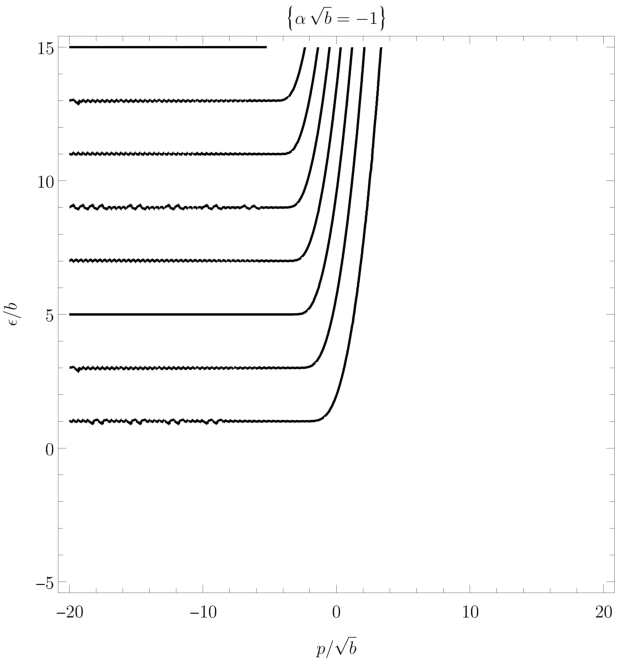
\includegraphics[width=0.45\textwidth]{grafy/robin-1.pdf}%
    \hspace{0.1\textwidth}%
    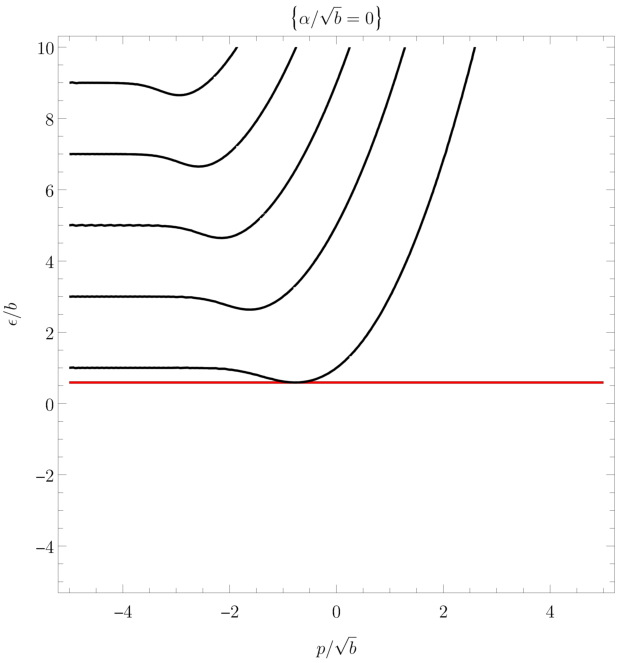
\includegraphics[width=0.45\textwidth]{grafy/robin0-degennes.pdf}%
    \\[1em]%
    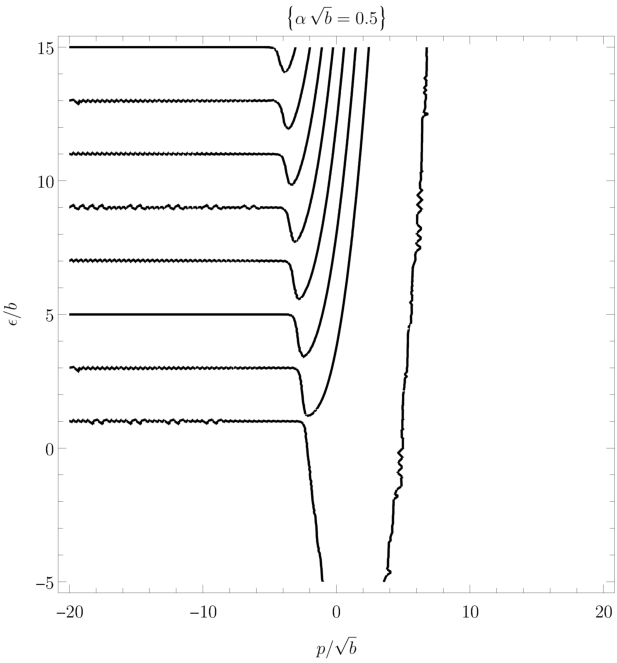
\includegraphics[width=0.45\textwidth]{grafy/robin0.5.pdf}%
    \hspace{0.1\textwidth}%
    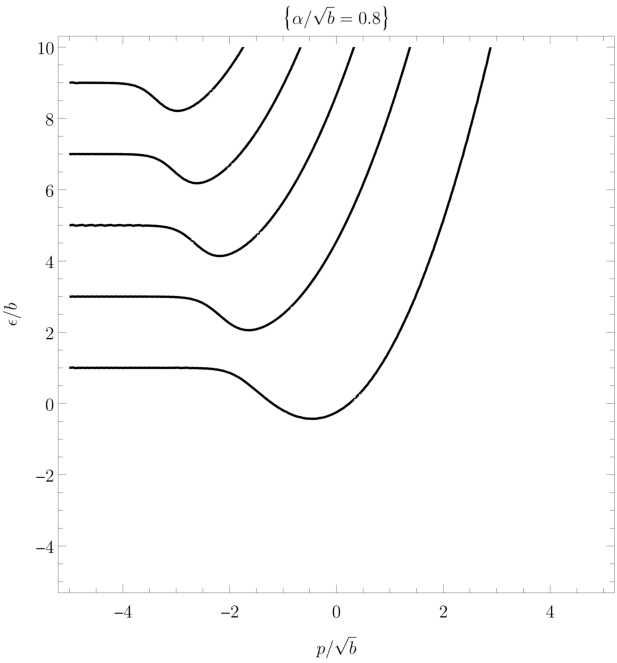
\includegraphics[width=0.45\textwidth]{grafy/robin0.8.pdf}%
    \\[1em]%
    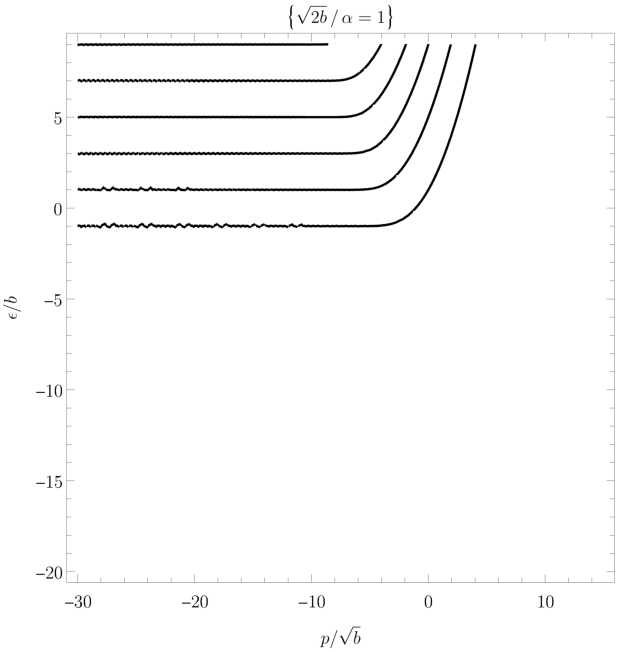
\includegraphics[width=0.45\textwidth]{grafy/robin1.pdf}%
    \hspace{0.1\textwidth}%
    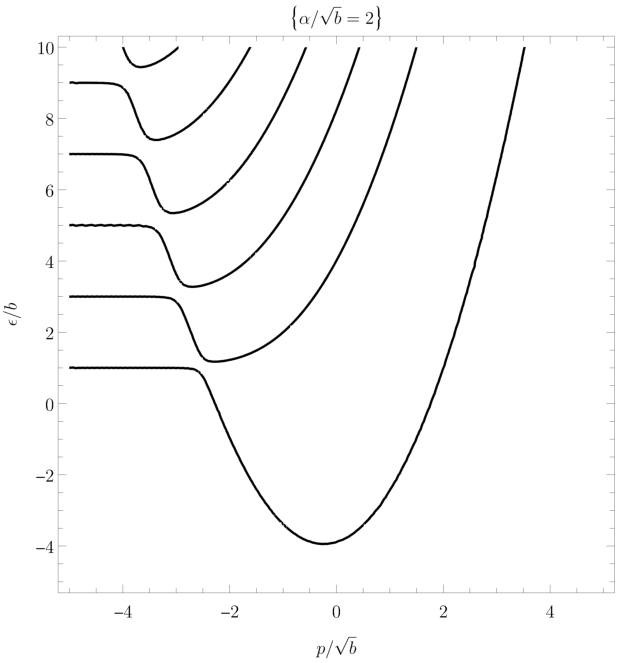
\includegraphics[width=0.45\textwidth]{grafy/robin2.pdf}\par
    \caption{The first energy levels $\epsilon$ as a function of the $y$-momentum $p$ for $\alpha\,\sqrt{b} = -1, \, 0, \, 0.5, \, 0.8, \, 1$ and $2$. The red line marks the predicted minimum $\epsilon = \Theta_0 \, b$.}
    \label{plots-robin}
\end{figure}

We are interested in the behaviour of $\epsilon_k(p)$ as $p \to \pm \infty$. The fibre Hamiltonian $\Hf_\alpha(p)$ with $p$ fixed is unitarily equivalent to a fibre Hamiltonian with $p=0$ translated by $p/b$, that is $\Hf_\alpha(p) \simeq T_{p/b} \, \Hf_\alpha(0) \, T_{-p/b}$, where $T_c \varphi(x) = {\varphi(x - c)}$. If~$p < 0$, this causes the Robin boundary to move to the left, away from the minimum of the effective potential. As $p \to -\infty$, the influence of the boundary decreases and the fibre Hamiltonian approaches that of a one-dimensional harmonic oscillator, hence $\epsilon_k \to b \, (2k+1)$. On the other hand, $p \to +\infty$ moves the boundary to the right, making increasingly larger areas with low effective potential forbidden, hence $\epsilon_k \to +\infty$.

These asymptotics make it clear that all energy levels above the lowest Landau level $\epsilon = b$ are allowed. However, one question still remains: what is the lowest allowed energy level? For the Neumann boundary ($\alpha = 0$), \cite{Noel2012} has proven the minimum energy to be
\begin{equation}
    \Theta_0
    \; := \;
    \min_{p \in \R \vph{\frac{1}{1}}}
    \frac{\epsilon_0(p)}{b}
    \: ,
    \qquad
    |\Theta_0 - 0.590106125|
    \leq 10^{-9}
    \: .
\end{equation}
The constant $\Theta_0$ is called the \textit{de Gennes constant} by some (e.g. \cite{ExnerLotoreichik2018}). For $\alpha > 0$ we will use the fact that the quadratic form of $\Hf_\alpha(p)$ is nonincreasing in $\alpha$. Let $\beta > \alpha$, then:
\begin{align*}
    \big( \varphi, \, \Hf_\alpha(p) \, \varphi \big)
    &= - \int_{\R_+} \overline\varphi \varphi''
    + \int_{\R_+} (bx+p)^2 |\varphi|^2
    \\[5pt]
    &= -\alpha \, |\varphi(0)|^2
    + \norm{\varphi'}_{L^2(\R_+)}
    + \norm{\varphi}_{L^2_{(bx+p)^2}(\R_+)}
    \\[5pt]
    &\geq -\beta \, |\varphi(0)|^2
    + \norm{\varphi'}_{L^2(\R_+)}
    + \norm{\varphi}_{L^2_{(bx+p)^2}(\R_+)}
    = \big( \varphi, \, \Hf_\beta(p) \, \varphi \big)
    \: .
    \numberthis\label{eqn-robin-form-monotonous}
\end{align*}
Therefore the minimum energy for $\Hf_\alpha(p), \, \alpha > 0$ will be less than $\Theta_0 \, b$.

For $\alpha < 0$, on the other hand, the inequality \eqref{eqn-robin-form-monotonous} implies that the minimum energy will be greater than $\Theta_0 \, b$. We will prove that it is still less than the lowest Landau level $b$. Searching for solutions of $F(...) = 0$ along $\epsilon = b$, we get:
\begin{align*}
    0 &=
    F(\alpha, \, p, \, \nu = 0)
    \\[5pt]
    0 &=
    \big( \alpha + p\big) \,
    D_0(p \, \sqrt{\tfrac{2}{b}})
    - \sqrt{2b} \,
    D_1(p \, \sqrt{\tfrac{2}{b}})
    \\[5pt]
    0 &=
    \big( \alpha + p\big) \,
    2^{-\frac{0}{2}} \,
    \e{-\frac{w^2}{4}} \,
    H_0\big( \frac{p}{\sqrt{b}} \big)
    \; - \;
    \sqrt{2b} \;
    2^{-\frac{1}{2}} \,
    \e{-\frac{w^2}{4}} \,
    H_1\big( \frac{p}{\sqrt{b}} \big)
    \\[5pt]
    0 &=
    \big( \alpha + p\big) \,
    H_0\big( \frac{p}{\sqrt{b}} \big)
    \; - \;
    \sqrt{b} \,
    H_1\big( \frac{p}{\sqrt{b}} \big)
    \\[5pt]
    0 &=
    \big( \alpha + p\big)
    \; - \;
    \sqrt{b} \;
    2 \; \frac{p}{\sqrt{b}}
    \\
    p &= \alpha
\end{align*}
Clearly, the solution always exists. It is straightforward to check that the sign of $F$ changes at $\alpha=p$, indicating that $\epsilon_0(p)$ actually \textit{crosses} the lowest Landau level. And since $\epsilon_0(p \to +\infty) \to +\infty$, the only way it can cross $\epsilon = b$ and still approach it as $p\to -\infty$ is by approaching it \textit{from below}. Thus, we have shown that $\min \epsilon_0(p) < b$.

Our estimate of the minimum energy for different values of $\alpha$ still leaves a lot to be desired. That is why we also computed a numerical approximation using \textit{mpmath} (see \cite{mpmath}). A table of the computed values and the code used to compute them is available in Section \ref{apdx-pythom} of the Appendix.

We have all the information needed to characterize the spectrum of $H_\alpha$ using Theorem~\ref{thm-direct-integral-spectrum}. Since neither of the energy functions is constant (they are analytic and grow indefinitely), the pure point spectrum of $H_\alpha$ is empty. Applying the result by \cite{Filonov2006}, we see that the singular continuous spectrum is empty too. What remains is the absolute continuous spectrum which goes from the energy minimum to infinity.

\section{Summary}
The following theorem summarizes the information we obtained about the spectrum of the Landau Hamiltonian in a half-plane with Robin boundary:
\begin{thm}
    Let $\alpha, \, b$ and $H_\alpha$ be as in Definition~\ref{defn-hamiltonian-robin}. If $\alpha > 0$, then there exists $E \in (-\infty, \Theta_0)$ such that $ \Sp(H_\alpha) = \SpAc(H_\alpha) = [E \, b, \; \infty )$.
    If $\alpha < 0$, then there exists $E \in (\Theta_0, 1)$ such that $\Sp(H_\alpha) = \SpAc(H_\alpha) = [E \, b, \; \infty )$.
    And finally, if $\alpha = 0$, then $\Sp(H_\alpha) = \SpAc(H_\alpha) = [\Theta_0 \, b, \; \infty )$. The value of $\Theta_0$ is $0.590106125 \pm 10^{-9}$.
\end{thm}


